% Options for packages loaded elsewhere
\PassOptionsToPackage{unicode}{hyperref}
\PassOptionsToPackage{hyphens}{url}
%
\documentclass[
]{article}
\usepackage{amsmath,amssymb}
\usepackage{lmodern}
\usepackage{ifxetex,ifluatex}
\ifnum 0\ifxetex 1\fi\ifluatex 1\fi=0 % if pdftex
  \usepackage[T1]{fontenc}
  \usepackage[utf8]{inputenc}
  \usepackage{textcomp} % provide euro and other symbols
\else % if luatex or xetex
  \usepackage{unicode-math}
  \defaultfontfeatures{Scale=MatchLowercase}
  \defaultfontfeatures[\rmfamily]{Ligatures=TeX,Scale=1}
\fi
% Use upquote if available, for straight quotes in verbatim environments
\IfFileExists{upquote.sty}{\usepackage{upquote}}{}
\IfFileExists{microtype.sty}{% use microtype if available
  \usepackage[]{microtype}
  \UseMicrotypeSet[protrusion]{basicmath} % disable protrusion for tt fonts
}{}
\makeatletter
\@ifundefined{KOMAClassName}{% if non-KOMA class
  \IfFileExists{parskip.sty}{%
    \usepackage{parskip}
  }{% else
    \setlength{\parindent}{0pt}
    \setlength{\parskip}{6pt plus 2pt minus 1pt}}
}{% if KOMA class
  \KOMAoptions{parskip=half}}
\makeatother
\usepackage{xcolor}
\IfFileExists{xurl.sty}{\usepackage{xurl}}{} % add URL line breaks if available
\IfFileExists{bookmark.sty}{\usepackage{bookmark}}{\usepackage{hyperref}}
\hypersetup{
  pdftitle={8th Protocol: Soil physics},
  pdfauthor={Cheyenne Rueda and Simone Massaro},
  hidelinks,
  pdfcreator={LaTeX via pandoc}}
\urlstyle{same} % disable monospaced font for URLs
\usepackage[margin=1in]{geometry}
\usepackage{color}
\usepackage{fancyvrb}
\newcommand{\VerbBar}{|}
\newcommand{\VERB}{\Verb[commandchars=\\\{\}]}
\DefineVerbatimEnvironment{Highlighting}{Verbatim}{commandchars=\\\{\}}
% Add ',fontsize=\small' for more characters per line
\usepackage{framed}
\definecolor{shadecolor}{RGB}{248,248,248}
\newenvironment{Shaded}{\begin{snugshade}}{\end{snugshade}}
\newcommand{\AlertTok}[1]{\textcolor[rgb]{0.94,0.16,0.16}{#1}}
\newcommand{\AnnotationTok}[1]{\textcolor[rgb]{0.56,0.35,0.01}{\textbf{\textit{#1}}}}
\newcommand{\AttributeTok}[1]{\textcolor[rgb]{0.77,0.63,0.00}{#1}}
\newcommand{\BaseNTok}[1]{\textcolor[rgb]{0.00,0.00,0.81}{#1}}
\newcommand{\BuiltInTok}[1]{#1}
\newcommand{\CharTok}[1]{\textcolor[rgb]{0.31,0.60,0.02}{#1}}
\newcommand{\CommentTok}[1]{\textcolor[rgb]{0.56,0.35,0.01}{\textit{#1}}}
\newcommand{\CommentVarTok}[1]{\textcolor[rgb]{0.56,0.35,0.01}{\textbf{\textit{#1}}}}
\newcommand{\ConstantTok}[1]{\textcolor[rgb]{0.00,0.00,0.00}{#1}}
\newcommand{\ControlFlowTok}[1]{\textcolor[rgb]{0.13,0.29,0.53}{\textbf{#1}}}
\newcommand{\DataTypeTok}[1]{\textcolor[rgb]{0.13,0.29,0.53}{#1}}
\newcommand{\DecValTok}[1]{\textcolor[rgb]{0.00,0.00,0.81}{#1}}
\newcommand{\DocumentationTok}[1]{\textcolor[rgb]{0.56,0.35,0.01}{\textbf{\textit{#1}}}}
\newcommand{\ErrorTok}[1]{\textcolor[rgb]{0.64,0.00,0.00}{\textbf{#1}}}
\newcommand{\ExtensionTok}[1]{#1}
\newcommand{\FloatTok}[1]{\textcolor[rgb]{0.00,0.00,0.81}{#1}}
\newcommand{\FunctionTok}[1]{\textcolor[rgb]{0.00,0.00,0.00}{#1}}
\newcommand{\ImportTok}[1]{#1}
\newcommand{\InformationTok}[1]{\textcolor[rgb]{0.56,0.35,0.01}{\textbf{\textit{#1}}}}
\newcommand{\KeywordTok}[1]{\textcolor[rgb]{0.13,0.29,0.53}{\textbf{#1}}}
\newcommand{\NormalTok}[1]{#1}
\newcommand{\OperatorTok}[1]{\textcolor[rgb]{0.81,0.36,0.00}{\textbf{#1}}}
\newcommand{\OtherTok}[1]{\textcolor[rgb]{0.56,0.35,0.01}{#1}}
\newcommand{\PreprocessorTok}[1]{\textcolor[rgb]{0.56,0.35,0.01}{\textit{#1}}}
\newcommand{\RegionMarkerTok}[1]{#1}
\newcommand{\SpecialCharTok}[1]{\textcolor[rgb]{0.00,0.00,0.00}{#1}}
\newcommand{\SpecialStringTok}[1]{\textcolor[rgb]{0.31,0.60,0.02}{#1}}
\newcommand{\StringTok}[1]{\textcolor[rgb]{0.31,0.60,0.02}{#1}}
\newcommand{\VariableTok}[1]{\textcolor[rgb]{0.00,0.00,0.00}{#1}}
\newcommand{\VerbatimStringTok}[1]{\textcolor[rgb]{0.31,0.60,0.02}{#1}}
\newcommand{\WarningTok}[1]{\textcolor[rgb]{0.56,0.35,0.01}{\textbf{\textit{#1}}}}
\usepackage{longtable,booktabs,array}
\usepackage{calc} % for calculating minipage widths
% Correct order of tables after \paragraph or \subparagraph
\usepackage{etoolbox}
\makeatletter
\patchcmd\longtable{\par}{\if@noskipsec\mbox{}\fi\par}{}{}
\makeatother
% Allow footnotes in longtable head/foot
\IfFileExists{footnotehyper.sty}{\usepackage{footnotehyper}}{\usepackage{footnote}}
\makesavenoteenv{longtable}
\usepackage{graphicx}
\makeatletter
\def\maxwidth{\ifdim\Gin@nat@width>\linewidth\linewidth\else\Gin@nat@width\fi}
\def\maxheight{\ifdim\Gin@nat@height>\textheight\textheight\else\Gin@nat@height\fi}
\makeatother
% Scale images if necessary, so that they will not overflow the page
% margins by default, and it is still possible to overwrite the defaults
% using explicit options in \includegraphics[width, height, ...]{}
\setkeys{Gin}{width=\maxwidth,height=\maxheight,keepaspectratio}
% Set default figure placement to htbp
\makeatletter
\def\fps@figure{htbp}
\makeatother
\setlength{\emergencystretch}{3em} % prevent overfull lines
\providecommand{\tightlist}{%
  \setlength{\itemsep}{0pt}\setlength{\parskip}{0pt}}
\setcounter{secnumdepth}{5}
\usepackage{fancyhdr}
\pagestyle{fancy}

\fancyhead[R]{Experimental bioclimatology}
\fancyfoot[L]{Cheyenne Rueda \& Simone Massaro}
\fancyfoot[R]{\thepage}
\fancyfoot[C]{}

% for having figures and tables staying in order
\usepackage{float}
\fancyhead[L]{Soil physics}
\usepackage{booktabs}
\usepackage{longtable}
\usepackage{array}
\usepackage{multirow}
\usepackage{wrapfig}
\usepackage{float}
\usepackage{colortbl}
\usepackage{pdflscape}
\usepackage{tabu}
\usepackage{threeparttable}
\usepackage{threeparttablex}
\usepackage[normalem]{ulem}
\usepackage{makecell}
\usepackage{xcolor}
\ifluatex
  \usepackage{selnolig}  % disable illegal ligatures
\fi
\newlength{\cslhangindent}
\setlength{\cslhangindent}{1.5em}
\newlength{\csllabelwidth}
\setlength{\csllabelwidth}{3em}
\newenvironment{CSLReferences}[2] % #1 hanging-ident, #2 entry spacing
 {% don't indent paragraphs
  \setlength{\parindent}{0pt}
  % turn on hanging indent if param 1 is 1
  \ifodd #1 \everypar{\setlength{\hangindent}{\cslhangindent}}\ignorespaces\fi
  % set entry spacing
  \ifnum #2 > 0
  \setlength{\parskip}{#2\baselineskip}
  \fi
 }%
 {}
\usepackage{calc}
\newcommand{\CSLBlock}[1]{#1\hfill\break}
\newcommand{\CSLLeftMargin}[1]{\parbox[t]{\csllabelwidth}{#1}}
\newcommand{\CSLRightInline}[1]{\parbox[t]{\linewidth - \csllabelwidth}{#1}\break}
\newcommand{\CSLIndent}[1]{\hspace{\cslhangindent}#1}

\title{8th Protocol: Soil physics}
\author{Cheyenne Rueda and Simone Massaro}
\date{21 junio 2021}

\begin{document}
\maketitle

{
\setcounter{tocdepth}{2}
\tableofcontents
}
\newpage

\hypertarget{motivation}{%
\section{Motivation}\label{motivation}}

During the previous protocols, it has been described that earth is formed by different atmospheric layers.
Well, is not only about these but also about the ones that are found more at the land surface.
Soil is the first layer found when land surface is reached.
It consists on the middle face between the lithosphere and the atmosphere.
Thus, soil is related with other factors, such as biology and hydrology.
Ecosystems are established on the soil, and soil is shaping them as the main source of resources for the natural habitats to expand (Lal and Shukla 2004).

Soil temperature and water content have a direct impact on two key process in the ecosystem: photosynthesis and respiration, which are basis of carbon dynamics. The former takes place in the canopy, but it requires the transpiration of water that comes from the soil. Moreover the soil temperature influences the leaves energy balance.
The majority of ecosystem respiration takes places in the soil (Yuste et al. 2005) and the soil temperature and humidity are the mail variables that control the soil respiration.
The respiration increases exponentially with temperature (Lloyd and Taylor 1994),
however at high temperature it is often limited by moisture (Orchard and Cook 1983).

In this report, the main focus is partly on soil heat storage and hydrology processes.

\hypertarget{background}{%
\section{Background}\label{background}}

Soil temperature and soil water content are both factors that alters soil respiration rate. Soil respiration is a process measured in \(\frac{\mu mol} {m^2 s}\) of \(CO_2\) (Courtois et al. 2018).
Soil is an important environmental variable partly in charge of an efficient ecosystem activity.
Soil moisture drives changes in stomata conductance, photosynthesis rate and energy partitioning. Water potential is the main reason of the movement of water through osmosis, gravity and air pressure.

Soil water potential is constitute by its matrix potential (adhesive force water-soil particles), osmotic potential (gradient of solute's {[}C{]}), pressure potential(pressure of air) and gravitational potential (mass of water).
REgarding water potential, other factors from the soil are very important.
These are its particles size, pore volume or pore size. This will variate depending on the type of soil at each moment, being sandy the soil with the thickest particles size with bigger pores and thus, less water retention capacity.

Soil characteristics can be approach by different perspectives, such as the surface energy fluxes and hydrology.
The first one regarding on the direct solar incoming radiation, reflected radiation and absorbed radiation.
The second one, regards on the precipitation, evaporation, infiltration, surface runoff. Each of these cause different processes on soil structure.

Going deeper into how energy fluxes affect the soil, the ground heat flux capacity will be introduced.
This process is based on Fourier's which describes the heat transfer in soil with the conduction of its components, from higher to lower temperatures.
In fact, this law includes parameters such as:

\begin{itemize}
\tightlist
\item
  \(k\): Thermal conductivity in \((W/mK)\)
\item
  \(T\) Temperature in \(K\)
\item
  \(z\) depth in \(m\)
\end{itemize}

The variation in soil temperature along a period of time depends in depth and the heat flux going inside it, as described by the following equation:
\[ T/t = 1/C_v [...]\]
\(C_v\): heat capacity in \((J m^{-3}K{-1})\)

The temperature along soil profile varies between day and night. During the day, the temperature of soil is higher than the temperature of air and thus starts to get more equally until night is set. After this occurs, the temperature of air is higher than the soil temperature, with this peak being more distinguish during midnight.

\hypertarget{sensors-and-measuring-principle}{%
\section{Sensors and measuring principle}\label{sensors-and-measuring-principle}}

\hypertarget{soil-hydrology}{%
\subsection{Soil hydrology}\label{soil-hydrology}}

For soil hydrology the main variable that are measured are the water content and the water potential.

To measure water content \textbf{time domain reflectrometry} it is used.
The principle behind this sensor is that the dielectric constant of the soil depends on the amount of water present.
The dielectric constant is estimated by measuring the travel time of a electromagnetic impulse between two rods inserted into the soil.

Water potential is measured using \textbf{tensionmeters}, that consists in a porous ceramic cap connect with a water reservoir under vacuum.
The has a low water potential therefore attracts the water from the tensiometer, until an equilibrium point is reached. By measuring the, negative, pressure in the water filled tube the water potential of the soil can be estimated.

\hypertarget{soil-tempertature}{%
\subsection{Soil tempertature}\label{soil-tempertature}}

Soil temperature is measured by \textbf{temperature sensors} placed a different depth.
Usually a resistance sensor, like the \emph{Pt100}, is used as long term stability is more important than high frequency response rate.
The presence of multiple temperature sensor along the soil profile allows also to estimate the soil heat fluxes.

Soil heat flux can also be directly measured using \textbf{heat flux plates}, which using a series of thermocouple estimated the amount of heat transferred between the hot and the cold side

\newpage

\hypertarget{analysis}{%
\section{Analysis}\label{analysis}}

\begin{Shaded}
\begin{Highlighting}[]
\FunctionTok{library}\NormalTok{(tidyverse)}
\end{Highlighting}
\end{Shaded}

\begin{verbatim}
## Warning: package 'tidyverse' was built under R version 4.0.5
\end{verbatim}

\begin{verbatim}
## Warning: package 'ggplot2' was built under R version 4.0.5
\end{verbatim}

\begin{verbatim}
## Warning: package 'tibble' was built under R version 4.0.5
\end{verbatim}

\begin{verbatim}
## Warning: package 'tidyr' was built under R version 4.0.5
\end{verbatim}

\begin{verbatim}
## Warning: package 'forcats' was built under R version 4.0.5
\end{verbatim}

\begin{Shaded}
\begin{Highlighting}[]
\FunctionTok{library}\NormalTok{(lubridate)}
\end{Highlighting}
\end{Shaded}

\begin{verbatim}
## Warning: package 'lubridate' was built under R version 4.0.5
\end{verbatim}

\begin{Shaded}
\begin{Highlighting}[]
\FunctionTok{library}\NormalTok{(FME)}
\FunctionTok{library}\NormalTok{(kableExtra)}
\end{Highlighting}
\end{Shaded}

\begin{verbatim}
## Warning: package 'kableExtra' was built under R version 4.0.5
\end{verbatim}

\begin{Shaded}
\begin{Highlighting}[]
\NormalTok{soil }\OtherTok{\textless{}{-}} \FunctionTok{read\_csv}\NormalTok{(}\StringTok{"../Data\_lectures/8\_Soil\_physics/Soil\_temperature\_bot\_garden.csv"}\NormalTok{)}
\end{Highlighting}
\end{Shaded}

\hypertarget{soil-heat-flux}{%
\subsection{Soil Heat flux}\label{soil-heat-flux}}

\emph{Calculate the soil heat flux in 5cm depth and the soil storage flux for the soil layer above from the soil temperature profile. Assume a thermal conductivity \(k=3.5 W/m K\) and a heat capacity \(c_p=3.5\times10^6 J/m^3K\). Compare your calculations with direct measurements of the soil heat flux. How do thermal conductivity and heat capacity affect your results?}

We proceed with the calculation of soil heat flux at 5cm depth, suing the temperature difference between 5 and 10 cm in soil. Also, soil heat storage will be calculated.

\begin{Shaded}
\begin{Highlighting}[]
\NormalTok{c2k }\OtherTok{\textless{}{-}} \ControlFlowTok{function}\NormalTok{(c) c }\SpecialCharTok{+} \FloatTok{273.15}
\NormalTok{k2c }\OtherTok{\textless{}{-}} \ControlFlowTok{function}\NormalTok{(k) k }\SpecialCharTok{{-}} \FloatTok{273.15}

\CommentTok{\#using as a reference the soil at 5 cm}
\NormalTok{d\_T\_space }\OtherTok{\textless{}{-}}\NormalTok{ soil}\SpecialCharTok{$}\NormalTok{Tsoil\_5cm\_degC }\SpecialCharTok{{-}}\NormalTok{ soil}\SpecialCharTok{$}\NormalTok{Tsoil\_10cm\_degC}
\NormalTok{d\_z\_space }\OtherTok{\textless{}{-}} \SpecialCharTok{{-}} \FloatTok{0.05} \CommentTok{\# m}


\NormalTok{d\_z\_time }\OtherTok{\textless{}{-}} \SpecialCharTok{{-}} \FloatTok{0.03} \CommentTok{\# m }
\NormalTok{d\_T\_time }\OtherTok{\textless{}{-}} \FunctionTok{c2k}\NormalTok{(}\FunctionTok{lag}\NormalTok{(soil}\SpecialCharTok{$}\NormalTok{Tsoil\_5cm\_degC)) }\SpecialCharTok{{-}} \FunctionTok{c2k}\NormalTok{(soil}\SpecialCharTok{$}\NormalTok{Tsoil\_5cm\_degC)}
\NormalTok{d\_t }\OtherTok{\textless{}{-}} \DecValTok{600} \CommentTok{\# seconds manually calculated from the dataset (10 min) }

\NormalTok{Cv }\OtherTok{\textless{}{-}} \FloatTok{3.5e6} \CommentTok{\# J m{-}3 K{-}1}
\NormalTok{k }\OtherTok{\textless{}{-}} \FloatTok{3.5} \CommentTok{\# W m{-}1 K{-}1}
\end{Highlighting}
\end{Shaded}

\begin{Shaded}
\begin{Highlighting}[]
\NormalTok{soil }\OtherTok{\textless{}{-}}\NormalTok{ soil }\SpecialCharTok{\%\textgreater{}\%} 
  \FunctionTok{mutate}\NormalTok{(}
    \AttributeTok{flux\_time =}\NormalTok{ d\_z\_time }\SpecialCharTok{*}\NormalTok{ d\_T\_time }\SpecialCharTok{*}\NormalTok{ Cv }\SpecialCharTok{/}\NormalTok{ d\_t, }\CommentTok{\# W m{-}2 }
    \AttributeTok{flux\_space =} \SpecialCharTok{{-}}\NormalTok{ k }\SpecialCharTok{*}\NormalTok{ (d\_T\_space }\SpecialCharTok{/}\NormalTok{ d\_z\_space), }\CommentTok{\# W m{-}2 }
    \AttributeTok{soil\_flux =}\NormalTok{ flux\_time }\SpecialCharTok{+}\NormalTok{ flux\_space)}
\end{Highlighting}
\end{Shaded}

\newpage

\begin{Shaded}
\begin{Highlighting}[]
\NormalTok{soil }\SpecialCharTok{\%\textgreater{}\%} 
  \FunctionTok{filter}\NormalTok{(}\FunctionTok{week}\NormalTok{(Date)}\SpecialCharTok{==}\DecValTok{15}\NormalTok{) }\SpecialCharTok{\%\textgreater{}\%} 
  \FunctionTok{ggplot}\NormalTok{(}\FunctionTok{aes}\NormalTok{(Date, soil\_flux)) }\SpecialCharTok{+}
  \FunctionTok{geom\_line}\NormalTok{(}\FunctionTok{aes}\NormalTok{(}\AttributeTok{col=}\StringTok{"Calculated"}\NormalTok{))}\SpecialCharTok{+}
  \FunctionTok{geom\_line}\NormalTok{(}\FunctionTok{aes}\NormalTok{(}\AttributeTok{y=}\NormalTok{SoilHeatFlux\_Wm2, }\AttributeTok{col=}\StringTok{"Measured"}\NormalTok{)) }\SpecialCharTok{+}
  \FunctionTok{scale\_colour\_manual}\NormalTok{(}\AttributeTok{values =} \FunctionTok{c}\NormalTok{(}\StringTok{"black"}\NormalTok{, }\StringTok{"\#F8766D"}\NormalTok{)) }\SpecialCharTok{+}
  \FunctionTok{labs}\NormalTok{(}\AttributeTok{y=}\StringTok{"Soil heat flux (W/m2)"}\NormalTok{, }\AttributeTok{col=}\StringTok{"Type heat flux"}\NormalTok{)}
\end{Highlighting}
\end{Shaded}

\begin{figure}
\centering
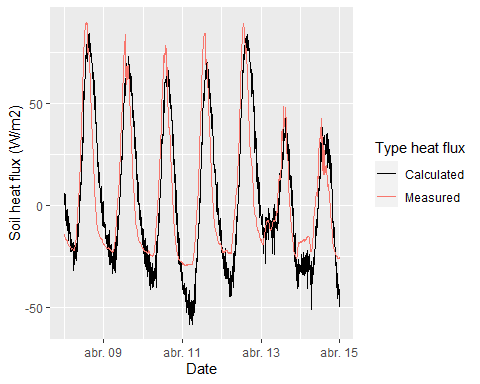
\includegraphics{8_soil_physics_files/figure-latex/soil-flux-1.pdf}
\caption{\label{fig:soil-flux}Comparison between heat flux measured (red) and calculated (black) over 1 week. Data collected at the botanical garden on the 8th-15th April 2021 at frequency of 10 minutes.}
\end{figure}

The heat flux measured at 5cm depth is compared with the one calculated in Figure \ref{fig:soil-flux}.
The two fluxes are overall comparable, with the exception of the early morning, when the measured flux stays constant at around -25 \(W/m^2\) while the calculated fluxes drops further.

\newpage

\hypertarget{influence-of-cv-and-k}{%
\subsubsection{Influence of Cv and K}\label{influence-of-cv-and-k}}

\begin{Shaded}
\begin{Highlighting}[]
\NormalTok{calc\_soil\_flux }\OtherTok{\textless{}{-}} \ControlFlowTok{function}\NormalTok{(pars)\{}
\NormalTok{  d\_T\_space }\OtherTok{\textless{}{-}}\NormalTok{ soil}\SpecialCharTok{$}\NormalTok{Tsoil\_5cm\_degC }\SpecialCharTok{{-}}\NormalTok{ soil}\SpecialCharTok{$}\NormalTok{Tsoil\_10cm\_degC}
\NormalTok{  d\_z\_space }\OtherTok{\textless{}{-}} \SpecialCharTok{{-}} \FloatTok{0.05}\CommentTok{\#m }
\NormalTok{  d\_z\_time }\OtherTok{\textless{}{-}} \SpecialCharTok{{-}} \FloatTok{0.03} \CommentTok{\# m }
\NormalTok{  d\_T\_time }\OtherTok{\textless{}{-}} \FunctionTok{c2k}\NormalTok{(}\FunctionTok{lag}\NormalTok{(soil}\SpecialCharTok{$}\NormalTok{Tsoil\_5cm\_degC)) }\SpecialCharTok{{-}} \FunctionTok{c2k}\NormalTok{(soil}\SpecialCharTok{$}\NormalTok{Tsoil\_5cm\_degC)}
\NormalTok{  flux\_time }\OtherTok{=}\NormalTok{ d\_z\_time }\SpecialCharTok{*}\NormalTok{ d\_T\_time }\SpecialCharTok{*}\NormalTok{ pars}\SpecialCharTok{$}\NormalTok{Cv }\SpecialCharTok{/}\NormalTok{ d\_t }\CommentTok{\# W m{-}2}
\NormalTok{  flux\_space }\OtherTok{=} \SpecialCharTok{{-}}\NormalTok{ pars}\SpecialCharTok{$}\NormalTok{k }\SpecialCharTok{*}\NormalTok{ (d\_T\_space }\SpecialCharTok{/}\NormalTok{ d\_z\_space) }\CommentTok{\# W m{-}2}
\NormalTok{  soil\_flux }\OtherTok{\textless{}{-}}\NormalTok{  flux\_time }\SpecialCharTok{+}\NormalTok{ flux\_space}
  \FunctionTok{tibble}\NormalTok{(}\AttributeTok{soil\_flux=}\NormalTok{soil\_flux[}\SpecialCharTok{{-}}\DecValTok{1}\NormalTok{]) }\CommentTok{\#remove first row that is NA}
\NormalTok{\}}
\NormalTok{pars }\OtherTok{\textless{}{-}} \FunctionTok{list}\NormalTok{(}\AttributeTok{Cv =} \FloatTok{3.6e6}\NormalTok{, }\AttributeTok{k=}\FloatTok{3.5}\NormalTok{)}
\NormalTok{sens }\OtherTok{\textless{}{-}} \FunctionTok{sensFun}\NormalTok{(calc\_soil\_flux, pars, }\AttributeTok{map=}\ConstantTok{NULL}\NormalTok{)}
\end{Highlighting}
\end{Shaded}

\begin{Shaded}
\begin{Highlighting}[]
\FunctionTok{summary}\NormalTok{(sens) }\SpecialCharTok{\%\textgreater{}\%} 
\NormalTok{  knitr}\SpecialCharTok{::}\FunctionTok{kable}\NormalTok{(}
    \AttributeTok{booktabs =} \ConstantTok{TRUE}\NormalTok{,}
    \AttributeTok{digits =} \DecValTok{2}\NormalTok{,}
    \AttributeTok{caption =} \StringTok{\textquotesingle{}Flux sensitivity\textquotesingle{}}
\NormalTok{  ) }\SpecialCharTok{\%\textgreater{}\%} 
  \FunctionTok{kable\_styling}\NormalTok{(}\AttributeTok{latex\_options =} \StringTok{"HOLD\_position"}\NormalTok{)}
\end{Highlighting}
\end{Shaded}

\begin{table}[H]

\caption{\label{tab:sens}Flux sensitivity}
\centering
\begin{tabular}[t]{lrrrrrrrr}
\toprule
  & value & scale & L1 & L2 & Mean & Min & Max & N\\
\midrule
Cv & 3.6e+06 & 3.6e+06 & 0.72 & 4.44 & 0.16 & -216.0 & 86.4 & 5500\\
k & 3.5e+00 & 3.5e+00 & 1.25 & 4.51 & 0.84 & -85.4 & 217.0 & 5500\\
\bottomrule
\end{tabular}
\end{table}

A local sensitivity analysis (Soetaert and Petzoldt 2010) was made for the two parameters used in the flux calculation: thermal conductivity (\(k\)) and heat capacity (\(C_v\)). The thermal conductivity has the biggest influence on the the overall flux (Table \ref{tab:sens}).

\newpage

\hypertarget{soil-temperature-profile}{%
\subsection{Soil temperature profile}\label{soil-temperature-profile}}

\emph{Visualize the soil temperature in different depths and discuss the temporal variability across one day.}

\begin{Shaded}
\begin{Highlighting}[]
\NormalTok{soil\_g }\OtherTok{\textless{}{-}}\NormalTok{ soil }\SpecialCharTok{\%\textgreater{}\%} 
  \FunctionTok{gather}\NormalTok{(}\StringTok{"depth"}\NormalTok{, }\StringTok{"T\_soil"}\NormalTok{, }\FunctionTok{starts\_with}\NormalTok{(}\StringTok{"Tsoil"}\NormalTok{)) }\SpecialCharTok{\%\textgreater{}\%} 
  \FunctionTok{mutate}\NormalTok{(}\AttributeTok{depth =} \FunctionTok{str\_extract}\NormalTok{(depth, }\StringTok{"}\SpecialCharTok{\textbackslash{}\textbackslash{}}\StringTok{d+"}\NormalTok{))}
\end{Highlighting}
\end{Shaded}

\begin{Shaded}
\begin{Highlighting}[]
\NormalTok{soil\_g }\SpecialCharTok{\%\textgreater{}\%} 
  \CommentTok{\# last day available to bet as close as possible to summer.}
  \CommentTok{\# Number 126 was got as \textasciigrave{}max(yday(soil$Date))\textasciigrave{}}
  \FunctionTok{filter}\NormalTok{(}\FunctionTok{yday}\NormalTok{(Date)}\SpecialCharTok{==}\DecValTok{126}\NormalTok{) }\SpecialCharTok{\%\textgreater{}\%} 
  \FunctionTok{ggplot}\NormalTok{(}\FunctionTok{aes}\NormalTok{(Date, T\_soil, }\AttributeTok{col=}\FunctionTok{as\_factor}\NormalTok{(depth))) }\SpecialCharTok{+}
  \FunctionTok{geom\_line}\NormalTok{() }\SpecialCharTok{+}
  \FunctionTok{labs}\NormalTok{(}\AttributeTok{y=}\StringTok{"Temperature soil (°C)"}\NormalTok{, }\AttributeTok{colour=}\StringTok{"Depth (cm)"}\NormalTok{)}
\end{Highlighting}
\end{Shaded}

\begin{figure}
\centering
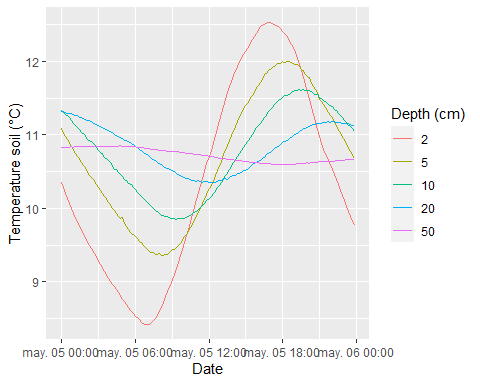
\includegraphics{8_soil_physics_files/figure-latex/profile-1.pdf}
\caption{\label{fig:profile}Soil temperature at different depths for one day. Data from 5th of May 2020, forest botanical garden.}
\end{figure}

The Figure \ref{fig:profile} shows the soil temperature for one day of may. It is possible to clearly see the difference of how at 0.5m depth the temperature of soil remains more stable regarding the other depths. During the changes of one day between day and night, at this depth the soil does not have enough time to change the temperature so fast.
The opposite is happening at a depth of 2cm or 5cm in soil, where the variations of temperature are stronger.
Just before the dawn in the morning, the soil reaches the lowest temperature values, between 8-9 °C at this depths.
Then during the day, the highest temperature is reached (12-13 °C) around 6pm where the sun starts going down starting the sunset.

\newpage

\hypertarget{references}{%
\section*{References}\label{references}}
\addcontentsline{toc}{section}{References}

\hypertarget{refs}{}
\begin{CSLReferences}{1}{0}
\leavevmode\hypertarget{ref-courtois_spatial_2018}{}%
Courtois, Elodie A., Clément Stahl, Joke Van den Berge, Laëtitia Bréchet, Leandro Van Langenhove, Andreas Richter, Ifigenia Urbina, Jennifer L. Soong, Josep Peñuelas, and Ivan A. Janssens. 2018. {``Spatial Variation of Soil {CO}2, {CH}4 and N2o Fluxes Across Topographical Positions in Tropical Forests of the Guiana Shield.''} \emph{Ecosystems} 21 (7): 1445--58. \url{https://doi.org/10.1007/s10021-018-0232-6}.

\leavevmode\hypertarget{ref-lal_principles_2004}{}%
Lal, Rattan, and Manoj K. Shukla. 2004. \emph{Principles of Soil Physics}. {CRC} Press.

\leavevmode\hypertarget{ref-lloyd_temperature_1994}{}%
Lloyd, J., and J. A. Taylor. 1994. {``On the Temperature Dependence of Soil Respiration.''} \emph{Functional Ecology} 8 (3): 315--23. \url{https://doi.org/10.2307/2389824}.

\leavevmode\hypertarget{ref-orchard_relationship_1983}{}%
Orchard, Valerie A., and F. J. Cook. 1983. {``Relationship Between Soil Respiration and Soil Moisture.''} \emph{Soil Biology and Biochemistry} 15 (4): 447--53. \url{https://doi.org/10.1016/0038-0717(83)90010-X}.

\leavevmode\hypertarget{ref-soetaert_inverse_2010}{}%
Soetaert, Karline, and Thomas Petzoldt. 2010. {``Inverse Modelling, Sensitivity and Monte Carlo Analysis in r Using Package {FME}.''} \emph{Journal of Statistical Software} 33 (1): 1--28. \url{https://doi.org/10.18637/jss.v033.i03}.

\leavevmode\hypertarget{ref-yuste_soil_2005}{}%
Yuste, J. Curiel, M. Nagy, I. A. Janssens, A. Carrara, and R. Ceulemans. 2005. {``Soil Respiration in a Mixed Temperate Forest and Its Contribution to Total Ecosystem Respiration.''} \emph{Tree Physiology} 25 (5): 609--19. \url{https://doi.org/10.1093/treephys/25.5.609}.

\end{CSLReferences}

\end{document}
